\apendice{Plan de Proyecto Software}

\section{Introducción}
Una de las fases más destacadas e imprescindible de un proyecto es la planificación. En esta fase se fijan los requisitos y se estima el tiempo y dinero que va a suponer la realización del proyecto.
Para esto, es necesario tener una idea global y a la vez concisa del proyecto que se va a realizar; de manera que ambas partes que forman el proyecto estén de acuerdo.

Así pues, vamos a dividir esta fase en dos apartados:

\begin{itemize}
\item
\textbf{Planificación temporal:} en este primer apartado se realizará una estimación de los tiempos esperados, así como fijar la fecha de inicio y fecha de fin del proyecto.
\item
\textbf{Estudio de viabilidad:} en este apartado se realizará un estudio de la viabilidad, es decir, ser capaces de apreciar si el proyecto ha sido exitoso o por el contrario ha sido un fracaso. 
\end{itemize}

Dentro de este último apartado se diferenciarán dos subapartados:

\begin{itemize}
\item
\textbf{Viabilidad económica:} se estimarán los costes y beneficios del proyecto.
\item
\textbf{Viabilidad legal:} se estudiarán las regulaciones legales que pudieran afectar al proyecto.
\end{itemize}


\section{Planificación temporal}
Para realizar una planificación correcta del proyecto, se decidió utilizar una metodología ágil de desarrollo, para ello se utilizó la metodología \emph{Scrum}. Como se explica en la memoria:

\begin{itemize}
	\item Se ha utilizado una estrategia orientada a un desarrollo incremental y basada en \emph{sprints}.
	\item La duración media de cada \emph{sprint} era aproximadamente de una semana.
	\item Al inicio de cada \emph{sprint} se definían las tareas o \emph{issues} a realizar, las cuales tenían que ser realizadas en un cierto intervalo de tiempo.
	\item Cada \emph{sprint} se planificaba cuando se finalizaban las tareas o \emph{issues} del anterior \emph{sprint}.	
	\item Al final de cada \emph{sprint} se revisan todas las tareas realizadas, así como ver si se han logrado los objetivos fijados y solucionado los problemas encontrados.
\end{itemize}

A continuación, se van a detallar los \emph{sprints} que se han realizado a lo largo del proyecto:

\subsection{Sprint 0 (25/02/19 - 10/03/19)}
En la primera reunión de planificación de proyecto se desarrollaron y expusieron las ideas del mismo. Además se propusieron las siguientes tareas:

\begin{itemize}
\item
\textbf{Crear repositorio de HitHub.} Además de crear el repositorio principal, se solicitó y posteriormente se adquirió \emph{Github Student Developer Pack}.
\item
\textbf{Descargar plantilla para la documentación}
\item
\textbf{Redactar los objetivos del proyecto}
\item
\textbf{Probar a leer archivos Excel con Python}  
\end{itemize}

Se estiman 12 horas de trabajo.


\subsection{Sprint 1 (11/03/19 - 17/03/19)}
En la segunda reunión se propusieron las siguientes tareas:

\begin{itemize}
\item
\textbf{Crear un algoritmo o proceso capaz de leer los archivos Excel.} En una tarea del anterior \emph{sprint} se apreció que no se podían leer los archivos Excel con Python, ya que los archivos tenían un error de formato y extensión. Por esta razón se optó por realizar un algoritmo que fuera capaz de leer estos archivos Excel(.xls) en modo texto, y parsear todo el contenido para generar otro archivo nuevo(.csv).
\end{itemize}

Se estiman 20 horas de trabajo.


\subsection{Sprint 2 (18/03/19 - 24/03/19)} 
En la tercera reunión se propusieron las siguientes tareas:

\begin{itemize}
\item
\textbf{Mejorar el algoritmo para leer los archivos Excel:} mejorar la expresión regular para que no fuera tan genérica y fuera más específica.
\item
\textbf{Redactar casos de uso 1 y 2}
\item
\textbf{Eliminar apartado \emph{Objetivos personales} de la documentación}
\item
\textbf{Descargar \emph{GitHub Desktop} y \emph{gVim 8.1}}
\end{itemize}

Se estiman 18 horas de trabajo.

\subsection{Sprint 3 (25/03/19 - 31/03/19)}
En la cuarta reunión se propusieron las siguientes tareas:

\begin{itemize}
\item
\textbf{Cambiar la forma de parsear los datos del algoritmo.} Obtener primero la información por filas, después por celdas y por último por DATA o contenido de las celdas. Pudiendo de esta manera obtener valores como \emph{MergeDown} y \emph{MergeAcross} que aportan información necesaria sobre la separación o combinación de celdas.   
\end{itemize}

Se estiman 20 horas de trabajo.

\subsection{Sprint 4 (01/04/19 - 07/04/19)}
En la quinta reunión se propusieron las siguientes tareas:

\begin{itemize}
\item
\textbf{Mejorar los nombres de variables del algoritmo}
\item
\textbf{Mejorar los casos de uso 1 y 2}
\item
\textbf{Redactar caso de uso 3}
\item
\textbf{Pensar si es necesario crear una Base de Datos y cómo crearla en tal caso}
\item
\textbf{Crear gráfico apilado horizontalmente(caso de uso 2)}
\end{itemize}

Se estiman 22 horas de trabajo.

\subsection{Sprint 5 (08/04/19 - 03/05/19)}
Hay que indicar que al coincidir con las vacaciones de Semana Santa, este \emph{sprint} tuvo una duración superior a una semana. En la sexta reunión se propusieron las siguientes tareas:

\begin{itemize}
\item
\textbf{Empezar a crear la interfaz gráfica.} Sacar un cuadro de diálogo cuando se pulse un botón de \emph{Cargar} que permita seleccionar ficheros.
\item
\textbf{Crear modelo Entidad-Relación}
\item
\textbf{Probar a entrecomillar los \emph{strings} de los (.csv) para poder leerlos bien}
\item
\textbf{Añadir apartado \emph{Planificación Temporal} en la Documentación}
\item
\textbf{Resolver problema con la obtención de la ruta.} Al seleccionar un fichero (mediante el cuadro de diálogo de la interfaz gráfica) se obtenía una ruta como la siguiente \emph{C:/Users/mdmar/Desktop/ficheroBueno.csv}, pero la ruta debería tener contrabarras o barras invertidas en vez de barras inclinadas.
\end{itemize}

Se estiman 45 horas de trabajo.

\subsection{Sprint 6 (04/05/19 - 07/05/19)}
En la séptima reunión (fue la primera videoconferencia que se realizó vía Skype) se propusieron las siguientes tareas:

\begin{itemize}
\item
\textbf{Añadir un \emph{Acerca de} en la interfaz gráfica.} Introducir escudo de la Universidad de Burgos, autor, tutor, fecha y versión.
\item
\textbf{Añadir líneas verticales al primer gráfico(apilado horizontal).} De esta manera se mejora la visualización del mismo.
\item
\textbf{Decidir si es necesario crear una pantalla de autenticación.} Incluso si se trata de una aplicación local, siempre es más seguro pedir la autenticación en caso de que dejemos el ordenador encendido.
\item
\textbf{Crear el logo de la aplicación} 
\item
\textbf{Seguir con la creación del modelo Entidad-Relación(Sprint 5)}
\end{itemize}

Se estiman 18 horas de trabajo.

\subsection{Sprint 7 (17/05/19 - 22/05/19)}
En la octava reunión (segunda videoconferencia que se realizó vía Skype) se propusieron las siguientes tareas:

\begin{itemize}
\item
\textbf{Cambiar el logo y el nombre del proyecto.} Poner un nombre menos genérico al proyecto.
\item
\textbf{Modificar el \emph{Acerca de} en la interfaz gráfica.} Recortar el pdf para que no se vea tanto espacio en blanco, añadir el logo y el nombre de la aplicación.
\item
\textbf{Automatizar las líneas verticales introducidas en el primer gráfico.} Tratar de automatizar las líneas verticales del primer gráfico, no introducirlas a mano una a una.
\item
\textbf{Crear el segundo gráfico.} Crear el segundo gráfico, indicando máximos, mínimos, medias y cuartiles de las asignaturas de cada curso de un año académico.
\end{itemize}

Se estiman 14 horas de trabajo.

\subsection{Sprint 8 (23/05/19 - 03/06/19)}
En la novena reunión (tercera videoconferencia que se realizó vía Skype) se propusieron las siguientes tareas:

\begin{itemize}
\item
\textbf{Crear Base de Datos(BBDD).} Crear la Base de Datos del proyecto, tal y como se define en el Modelo Entidad-Relación creado.
\item
\textbf{Añadir el \emph{Modelo ER} y las \emph{tablas a crear} en la Documentación.}
\item
\textbf{Crear otro tipo/modelo de gráfico, similar al segundo gráfico.} En vez de asignaturas por cada curso de un año, que se visualicen asignaturas por cada semestre de un año. Es decir, visualizar el doble de columnas(8) o de cajas que en el segundo gráfico(4).
\item
\textbf{Buscar información sobre cómo comparar gráficos en \emph{Python}.}
\end{itemize}

Se estiman 25 horas de trabajo.

\subsection{Sprint 9 (04/06/19 - 10/06/19)}
En la décima reunión (cuarta videoconferencia que se realizó vía Skype) se propusieron las siguientes tareas:

\begin{itemize}
\item
\textbf{Permitir carga de datos de fichero con múltiples titulaciones.} Permitir que el sistema pueda cargar datos en la BBDD a partir de un fichero con múltiples titulaciones.
\item
\textbf{Crear casos de usos para los botones de Crear BBDD, Cargar Datos y Salir.}
\item
\textbf{Cambiar Botón de Crear BBDD a menú superior.} Es un botón o función que se utilizará con poca frecuencia, ya que una vez creada la BBDD, no hará falta volverla a crear.
\item
\textbf{Pensar el modo de permitir seleccionar las gráficas al usuario.} Lista jerárquica, lista desplegable... etc.
\item
\textbf{Arreglar problema de la Documentación con la barra baja(\_) en Latex}
\end{itemize}

Se estiman 28 horas de trabajo.

\subsection{Sprint 10 (11/06/19 - 18/06/19)}
En la undécima reunión (quinta videoconferencia que se realizó vía Skype) se propusieron las siguientes tareas:

\begin{itemize}
\item
\textbf{Mejorar \emph{Introducción}, hacer \emph{Resumen} y \emph{Palabras Clave}.}
\item
\textbf{Mejorar apartado \emph{C.2. Diseño de datos} de los anexos.} También girar imagen de modelo ER, cambiar posición de imágenes de la BBDD...).
\item
\textbf{Crear caso de uso para el boton de \emph{Preprocesado}.}
\item
\textbf{Crear y diferenciar 2 botones en la interfaz gráfica (\emph{Preprocesado} y \emph{Cargar Archivos}).} 
\item
\textbf{Crear 3 botones (con una imagen cada uno) en la interfaz gráfica.} Para poder seleccionar el tipo de gráfico.
\item
\textbf{Hacer \emph{Técnicas y Herramientas} de la memoria.}
\item
\textbf{Hacer \emph{C.3. Diseño procedimental} y \emph{C.4. Diseño arquitectónico} de los anexos.}
\end{itemize}

Se estiman 35 horas de trabajo.


\subsection{Sprint 11 (19/06/19 - 25/06/19)}
En la duodécima reunión (sexta videoconferencia que se realizó vía Skype) se propusieron las siguientes tareas:

\begin{itemize}
\item
\textbf{Mejorar traducción del \emph{Resumen}.}
\item
\textbf{Hacer \emph{Conceptos teóricos} de la memoria.}
\item
\textbf{Obtener los gráficos en cada ventana de los diferentes tipos de gráficos.} Obtener los gráficos creados a partir de la información de la BBDD y de lo que haya seleccionado el usuario.
\item
\textbf{Añadir botón de \emph{Descargar Gráfico}.} El botón permitirá descargar el gráfico como una imagen (.png) en la ruta donde se encuentre la aplicación.
\item
\textbf{Crear un diagrama UML con todos los casos de uso.}
\end{itemize}

Se estiman 40 horas de trabajo.

\subsection{Sprint 12 (26/06/19 - 01/07/19)}

En la decimotercera reunión (séptima videoconferencia que se realizó vía Skype) se propusieron las siguientes tareas:

\begin{itemize}
\item
\textbf{Finalizar la interfaz gráfica.}
\item
\textbf{Crear un ejecutable para poder ejecutar la aplicación.}
\item
\textbf{Mejorar tamaño de imágenes y pies de página en la documentación.}
\item
\textbf{Descargar los gráficos visualizando toda la información.} Evitar que al descargar las imágenes de los gráficos, por defecto se corten los nombres de las asignaturas.
\item
\textbf{Finalizar los anexos.}
\item
\textbf{Finalizar la memoria.}
\end{itemize}

Se estiman 45 horas de trabajo.

\subsection{Resumen}
En la siguiente tabla se puede apreciar el tiempo dedicado a cada tarea:


\begin{longtable}[]{@{}lrr@{}}
\toprule
\begin{minipage}[b]{0.37\columnwidth}\raggedright\strut
Tarea\strut
\end{minipage} & \begin{minipage}[b]{0.37\columnwidth}\raggedleft\strut
Tiempo (horas)\strut
\end{minipage}\tabularnewline
\midrule
\endhead

\begin{minipage}[t]{0.37\columnwidth}\raggedright\strut
\emph{Programación}\strut
\end{minipage} & \begin{minipage}[t]{0.37\columnwidth}\raggedleft\strut
140\strut
\end{minipage}\tabularnewline
\begin{minipage}[t]{0.37\columnwidth}\raggedright\strut
\emph{Documentación}\strut
\end{minipage} & \begin{minipage}[t]{0.37\columnwidth}\raggedleft\strut
80\strut
\end{minipage}\tabularnewline
\begin{minipage}[t]{0.37\columnwidth}\raggedright\strut
\emph{Investigación}\strut
\end{minipage}& \begin{minipage}[t]{0.37\columnwidth}\raggedleft\strut
70\strut
\end{minipage}\tabularnewline
\begin{minipage}[t]{0.37\columnwidth}\raggedright\strut
\emph{Corrección de errores}\strut
\end{minipage} & \begin{minipage}[t]{0.37\columnwidth}\raggedleft\strut
52\strut
\end{minipage}\tabularnewline
\begin{minipage}[t]{0.37\columnwidth}\raggedright\strut
\emph{Reuniones de seguimiento}\strut
\end{minipage} & \begin{minipage}[t]{0.37\columnwidth}\raggedleft\strut
13\strut
\end{minipage}\tabularnewline
\midrule
\begin{minipage}[t]{0.37\columnwidth}\raggedright\strut
Total\strut
\end{minipage} & \begin{minipage}[t]{0.37\columnwidth}\raggedleft\strut
355\strut
\end{minipage}\tabularnewline
\bottomrule
\caption{Horas empleadas en el proyecto.}
\end{longtable}

En la figura \ref{fig:resumenHoras} se puede apreciar un gráfico sobre la distribución del tiempo empleado durante el desarrollo del proyecto.

\begin{figure}%[!h]
		\centering
		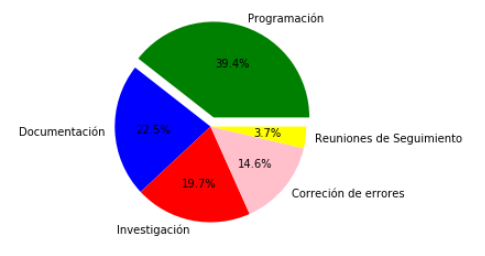
\includegraphics[width=0.9\textwidth]{resumenHoras}
		\caption{Gráfico con el resumen de las horas empleadas en el proyecto}\label{fig:resumenHoras}
	\end{figure}


\subsection{Gráficos y estadísticas}

Con la ayuda de los datos que ofrece GitHub, se van a visualizar una serie de gráficos sobre el desarrollo del proyecto.


\begin{itemize}
\item \textbf{Commits.} En la figura \ref{fig:commits} se aprecia un gráfico de barras, donde se muestra la cantidad de  \emph{commits} que se ha realizado cada semana.
\item \textbf{Contribuciones.} En la gráfica de la figura \ref{fig:contribuconesConstantes} se aprecia que el desarrollo del proyecto ha sido constante, con numerosos \emph{issues}, \emph{commits} y aportaciones a lo largo de los cuatro meses.
\end{itemize}

\begin{figure}%[!h]
		\centering
		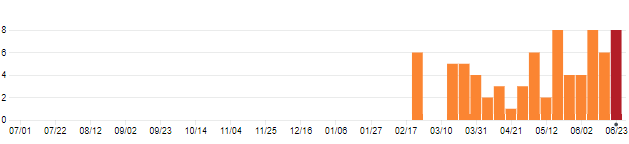
\includegraphics[width=\textwidth]{commits}
		\caption{Gráfico con los \emph{commits} que se ha realizado cada semana}\label{fig:commits}
	\end{figure}

\begin{figure}%[!h]
		\centering
		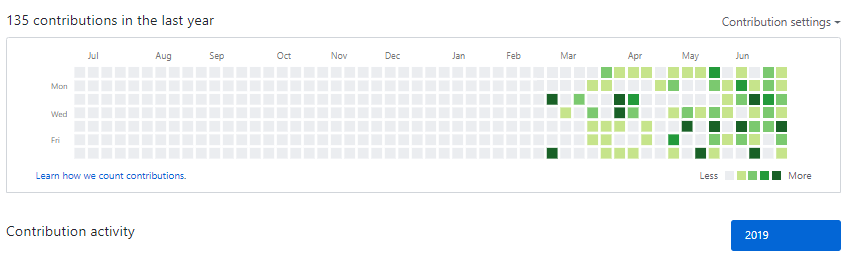
\includegraphics[width=\textwidth]{contribuconesConstantes}
		\caption{Gráfico donde se aprecia el desarrollo constante}\label{fig:contribuconesConstantes}
	\end{figure}

\section{Estudio de viabilidad}
En este apartado se va a analizar tanto la viabilidad económica como la viabilidad legal del proyecto.


\subsection{Viabilidad económica} 
En este subapartado se van a exponer los costes y beneficios que hubiera tenido el desarrollo del proyecto en un entorno empresarial real. 

\begin{itemize}
	\item\textbf{Costes de personal:}

El proyecto ha sido realizado por una única persona (desarrollador junior a tiempo completo) durante un total de tres meses.
De acuerdo a lo anterior, se consideran los siguientes valores:

\begin{longtable}[]{@{}lr@{}}
\toprule
\begin{minipage}[b]{0.38\columnwidth}\raggedright\strut
\textbf{Concepto}\strut
\end{minipage} & \begin{minipage}[b]{0.20\columnwidth}\raggedleft\strut
\textbf{Coste (\euro{}) }\strut
\end{minipage}\tabularnewline
\midrule
\endhead
\begin{minipage}[t]{0.38\columnwidth}\raggedright\strut
Salario anual bruto\strut
\end{minipage} & \begin{minipage}[t]{0.20\columnwidth}\raggedleft\strut
{18000}\strut
\end{minipage}\tabularnewline
\begin{minipage}[t]{0.38\columnwidth}\raggedright\strut
Coste S.Social empresa (36\%)\strut
\end{minipage} & \begin{minipage}[t]{0.20\columnwidth}\raggedleft\strut
6480\strut
\end{minipage}\tabularnewline
\midrule
\begin{minipage}[t]{0.38\columnwidth}\raggedright\strut
\textbf{Coste Total anual}\strut
\end{minipage} & \begin{minipage}[t]{0.20\columnwidth}\raggedleft\strut
24480\strut
\end{minipage}\tabularnewline
\bottomrule
\caption{Costes de personal anual.}
\end{longtable}


Por lo tanto, el precio por hora se calcula dividiendo el \emph{Coste Total anual} entre la jornada anual estimada de 1700 horas. Luego se obtiene un precio de 14.40\euro{} la hora. Como anteriormente se han estimado 355 horas de realización del proyecto, se obtiene un coste total de 5112\euro{}. 
Hay que destacar que a este coste habría que añadirle el coste del tutor. 

\newpage

\item\textbf{Costes de hardware:}
Para la realización de este proyecto se ha utilizado un ordenador portátil que tiene una antigüedad aproximada de 4 años y 
se estima un valor aproximado de 800\euro{}. El tiempo utilizado ha sido de 4 meses, luego el coste amortizado durante estos meses sería de 48\euro{}.




\item\textbf{Costes de software:}
Para la realización del proyecto todas las herramientas y programas utilizados han sido de software libre y gratuito. Las herramientas que no cumplían estas características, se optó por utilizar su versión de prueba (\emph{Nitro Pro} por ejemplo).




\item\textbf{Costes totales:}
La suma total de todos los costes anteriores es la siguiente:


\begin{longtable}[]{@{}lr@{}}
\toprule
\begin{minipage}[b]{0.22\columnwidth}\raggedright\strut
\textbf{Concepto}\strut
\end{minipage} & \begin{minipage}[b]{0.22\columnwidth}\raggedright\strut
\textbf{Coste}\strut
\end{minipage}\tabularnewline
\midrule
\endhead
\begin{minipage}[t]{0.22\columnwidth}\raggedright\strut
\emph{Personal}\strut
\end{minipage} & \begin{minipage}[t]{0.22\columnwidth}\raggedright\strut
5112\euro{}\strut
\end{minipage}\tabularnewline
\begin{minipage}[t]{0.22\columnwidth}\raggedright\strut
\emph{Hardware}\strut
\end{minipage} & \begin{minipage}[t]{0.22\columnwidth}\raggedright\strut
48\euro{}\strut
\end{minipage}\tabularnewline
\begin{minipage}[t]{0.22\columnwidth}\raggedright\strut
Software\strut
\end{minipage} & \begin{minipage}[t]{0.22\columnwidth}\raggedright\strut
0\euro{}\strut
\end{minipage}\tabularnewline
\midrule
\begin{minipage}[t]{0.22\columnwidth}\raggedright\strut
Total\strut
\end{minipage} & \begin{minipage}[t]{0.22\columnwidth}\raggedright\strut
5160\euro{}\strut
\end{minipage}\tabularnewline
\bottomrule
\caption{Costes totales.}
\end{longtable}


Teniendo en cuenta los datos obtenidos anteriormente, se concluye que para que el proyecto resulte rentable en el período aproximado de uno o dos años, sería necesario utilizar la aplicación para la generación de las diferentes gráficas en todas las titulaciones de la Universidad de Burgos que lo consideraran adecuado. 

De esta manera se amortizaría la aplicación, ya que vender licencias de la misma, no tiene mucho sentido en un entorno externo a la universidad.
No se establece una periodicidad del uso de la aplicación, ya que podría ser utilizada en diferentes momentos del curso académico al poder almacenar datos de años anteriores, así como datos de matriculación del año actual. 

\end{itemize}

\subsection{Viabilidad legal}

A continuación se expone la viabilidad del proyecto en el ámbito legal, es decir, las licencias del software utilizado en el desarrollo de mismo. 

El lenguaje de programación \emph{Python} y todos sus módulos y librerías, poseen la licencia \emph{PSFL(Python Software Foundation License)}\cite{python}. Este tipo de licencia, es exclusivo de \emph{Python} y cumple con los requisitos \emph{OSI}\footnote{Open Source Initiative}, por lo tanto es categorizada dentro de las licencias de software libre.


Todas las herramientas que se han utilizado han sido de software libre, como se ha comentado en la memoria en el apartado de \emph{Técnicas y herramientas}.


Por lo tanto, teniendo en cuenta las licencias de las herramientas utilizadas, la licencia que mejor se ajusta a nuestro proyecto es la \emph{GNU (General Public License)}\cite{gnu} en su última versión (versión 3).





